\tikzset{every picture/.style={line width=0.75pt}} %set default line width to 0.75pt        

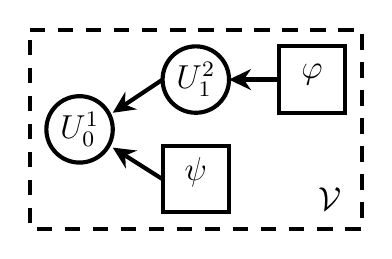
\begin{tikzpicture}[x=0.6pt,y=0.6pt,yscale=-1,xscale=1]
%uncomment if require: \path (0,300); %set diagram left start at 0, and has height of 300

%Shape: Circle [id:dp821654118938725] 
\draw  [line width=1.5]  (130,70) .. controls (130,58.95) and (138.95,50) .. (150,50) .. controls (161.05,50) and (170,58.95) .. (170,70) .. controls (170,81.05) and (161.05,90) .. (150,90) .. controls (138.95,90) and (130,81.05) .. (130,70) -- cycle ;
%Shape: Circle [id:dp9693294242254202] 
\draw  [line width=1.5]  (200,40) .. controls (200,28.95) and (208.95,20) .. (220,20) .. controls (231.05,20) and (240,28.95) .. (240,40) .. controls (240,51.05) and (231.05,60) .. (220,60) .. controls (208.95,60) and (200,51.05) .. (200,40) -- cycle ;
%Straight Lines [id:da2336152744929989] 
\draw [line width=1.5]    (200,100) -- (173.38,83.14) ;
\draw [shift={(170,81)}, rotate = 392.35] [fill={rgb, 255:red, 0; green, 0; blue, 0 }  ][line width=0.08]  [draw opacity=0] (13.4,-6.43) -- (0,0) -- (13.4,6.44) -- (8.9,0) -- cycle    ;
%Straight Lines [id:da7555295343349109] 
\draw [line width=1.5]    (200,40) -- (173.33,57.78) ;
\draw [shift={(170,60)}, rotate = 326.31] [fill={rgb, 255:red, 0; green, 0; blue, 0 }  ][line width=0.08]  [draw opacity=0] (13.4,-6.43) -- (0,0) -- (13.4,6.44) -- (8.9,0) -- cycle    ;
%Shape: Rectangle [id:dp057979059306741076] 
\draw  [dash pattern={on 5.63pt off 4.5pt}][line width=1.5]  (120,10) -- (320,10) -- (320,130) -- (120,130) -- cycle ;
%Shape: Rectangle [id:dp30596298266066313] 
\draw  [line width=1.5]  (270,20) -- (310,20) -- (310,60) -- (270,60) -- cycle ;
%Shape: Rectangle [id:dp9621262435565225] 
\draw  [line width=1.5]  (200,80) -- (240,80) -- (240,120) -- (200,120) -- cycle ;
%Straight Lines [id:da8176933026073245] 
\draw [line width=1.5]    (270,40) -- (244,40) ;
\draw [shift={(240,40)}, rotate = 360] [fill={rgb, 255:red, 0; green, 0; blue, 0 }  ][line width=0.08]  [draw opacity=0] (13.4,-6.43) -- (0,0) -- (13.4,6.44) -- (8.9,0) -- cycle    ;

% Text Node
\draw (150,70) node  [font=\large]  {$U_{0}^{1}$};
% Text Node
\draw (220,40) node  [font=\large]  {$U_{1}^{2}$};
% Text Node
\draw (290,37) node  [font=\large]  {$\varphi $};
% Text Node
\draw (220,96) node  [font=\large]  {$\psi $};
% Text Node
\draw (301,112) node  [font=\large]  {$\mathcal{V}$};


\end{tikzpicture}
